%%%%%%%%%%%%%%%%%%%%%%%%%%%%%%%%%%%%%%%%%%%%%%%%%%%%%%%%%%%%%%%%%%%%%%%%%%%%%%%%%%%%%%%%%%%%
%%
%% Chapter 2 : Background
%%
%%      * Should give the necessary info/math/tools to understand the proposal
%%
%%  BASIC STRUCTURE :
%%
%%      a. DRL overview
%%            * RL definition
%%            * RL mathematical problem formulation
%%            * RL methods
%%              > Value based methods
%%                  - Exact methods using DP (planning by DP)
%%                  - Model free prediction (MonteCarlo and TD learning)
%%                  - Model free control (MonteCarlo, SARSA and Q-learning)
%%              > Policy based methods
%%                  - Policy gradients
%%                  - Actor Critic methods
%%            * RL with function approximation
%%            * DeepRL overview (DQN, PPO)
%%
%%      b. Simulated environments (talk about ALE, Gym)
%%          * Why is this important?
%%          * Some success stories
%%
%%      c. Simulated environments for robot locomotion
%%          * Physics engines
%%          * Robot representations
%%              - Kinematic trees
%%              - Model formats (urdf,mjcf,sdf)
%%              - Actuation models
%%          * Generic framework architecture
%%
%%%%%%%%%%%%%%%%%%%%%%%%%%%%%%%%%%%%%%%%%%%%%%%%%%%%%%%%%%%%%%%%%%%%%%%%%%%%%%%%%%%%%%%%%%%%
\chapter{Background}
\label{ch:background}

%%%%%%%%%%%%%%%%%%%%%%%%%%%%%%%
%   Figures for chapter 2
%%%%%%%%%%%%%%%%%%%%%%%%%%%%%%%

\newcommand{\figrlloop}{
    \begin{figure}
        \centering
        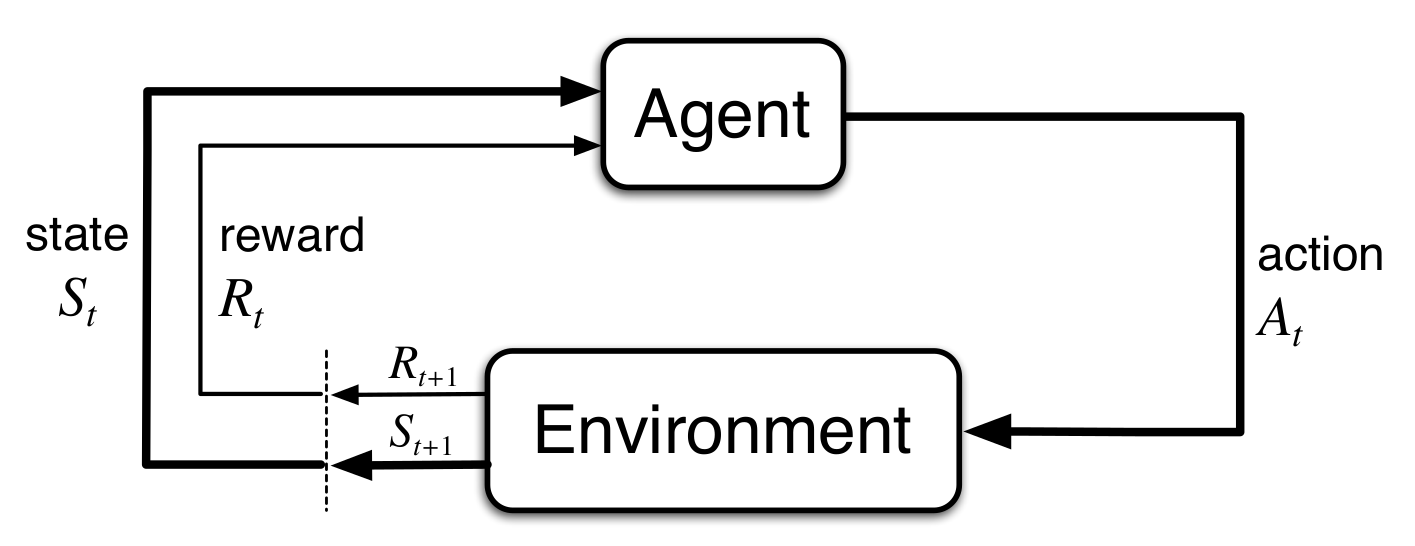
\includegraphics[width=5in]{./chapters/chapter_2/imgs/img_rl_loop.png}
        \caption{Agent-Environment interaction loop}
        \label{fig:ch2_rlloop}
    \end{figure}
}

\newcommand{\figdrlsamplesFirst}{
    \begin{figure}
        \centering
        \begin{subfigure}[b]{0.4\textwidth}
            \centering
            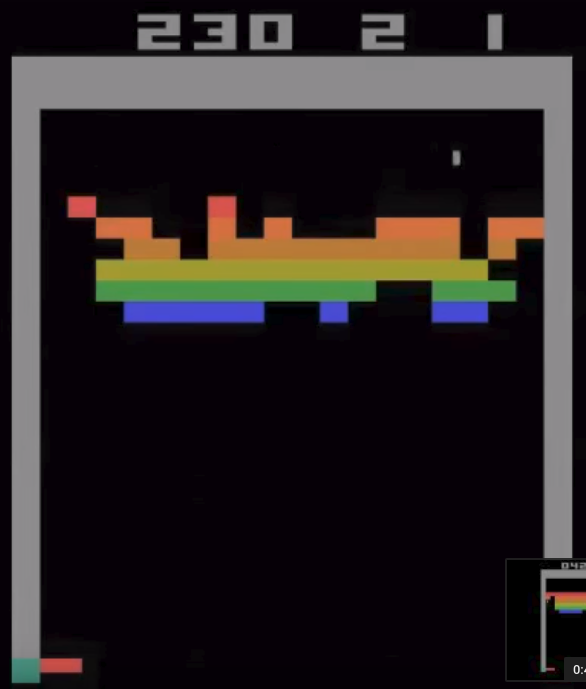
\includegraphics[width=0.9\textwidth]{./chapters/chapter_2/imgs/img_dqn_breakout.png}
            \caption{}
            \label{fig:ch2_dqn_breakout}
        \end{subfigure}
        \begin{subfigure}[b]{0.4\textwidth}
            \centering
            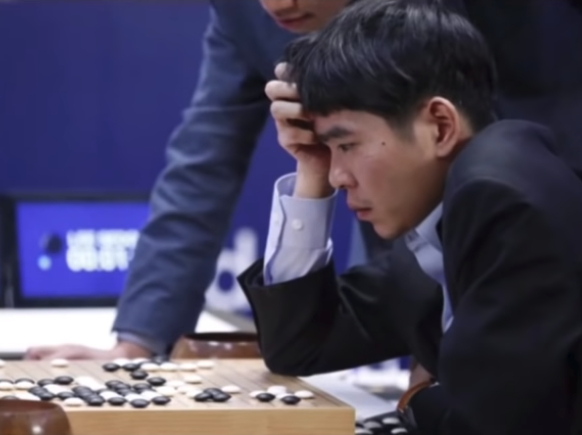
\includegraphics[width=0.9\textwidth]{./chapters/chapter_2/imgs/img_alphago.png}
            \caption{}
            \label{fig:ch2_alphago}
        \end{subfigure}
        \caption{Some DeepRL success stories: (a) DQN agent playing atari breakout [@CITE],
                                              (b) AlphaGo playing against Go champion Lee Sedol [@CITE]}
        \label{fig:ch2_drl_stories_1}
    \end{figure}
}

\newcommand{\figdrlsamplesSecond}{
    \begin{figure}
        \centering
        \begin{subfigure}[b]{0.3\textwidth}
            \centering
            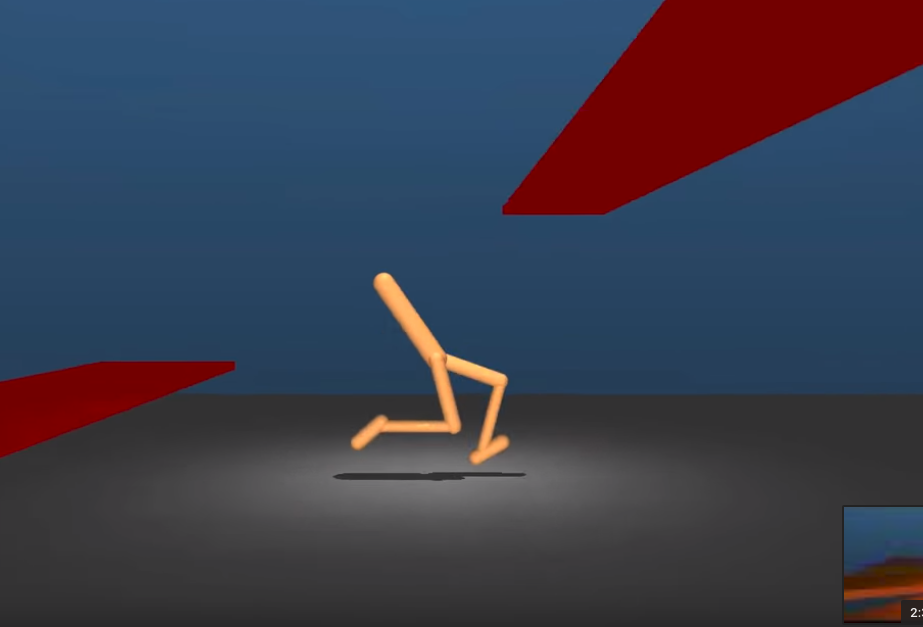
\includegraphics[width=0.9\textwidth]{./chapters/chapter_2/imgs/img_emergence_of_locomotion.png}
            \caption{}
            \label{fig:ch2_emergence_of_locomotion}
        \end{subfigure}
        \begin{subfigure}[b]{0.3\textwidth}
            \centering
            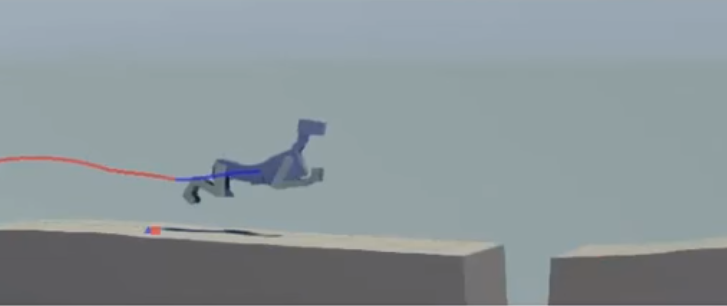
\includegraphics[width=0.9\textwidth]{./chapters/chapter_2/imgs/img_deepterrainrl.png}
            \caption{}
            \label{fig:ch2_deepterrainrl}
        \end{subfigure}
        \begin{subfigure}[b]{0.3\textwidth}
            \centering
            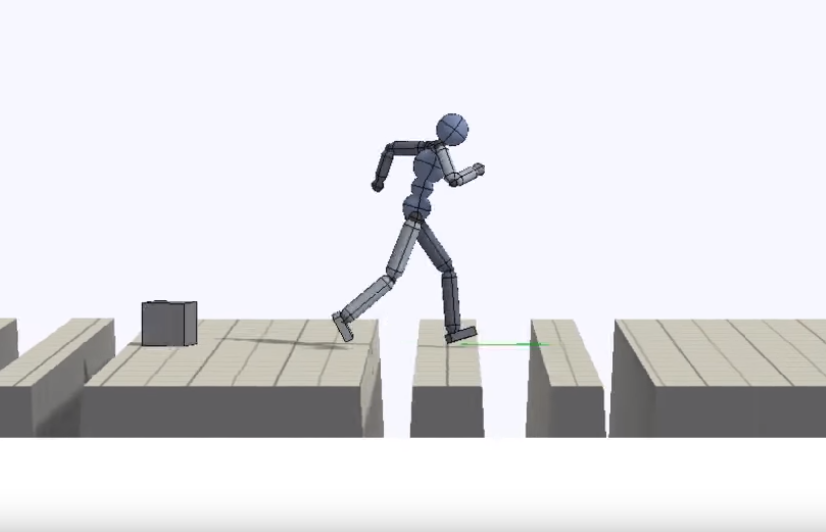
\includegraphics[width=0.9\textwidth]{./chapters/chapter_2/imgs/img_deepmimic.png}
            \caption{}
            \label{fig:ch2_deepmimic}
        \end{subfigure}
        \caption{Some DeepRL success stories: (a) Deepmind's agent running in a simulated environment [@CITE],
                                              (b) Simulated dog running in a course with obstacles [@CITE],
                                              (c) Simulated character running in an obstacle course, while 
                                                  mimicking humans' natural motion [@CITE]}
        \label{fig:ch2_drl_stories_2}
    \end{figure}
}

\newcommand{\figdrlsamplesThird}{
    \begin{figure}
        \centering
        \begin{subfigure}[b]{0.3\textwidth}
            \centering
            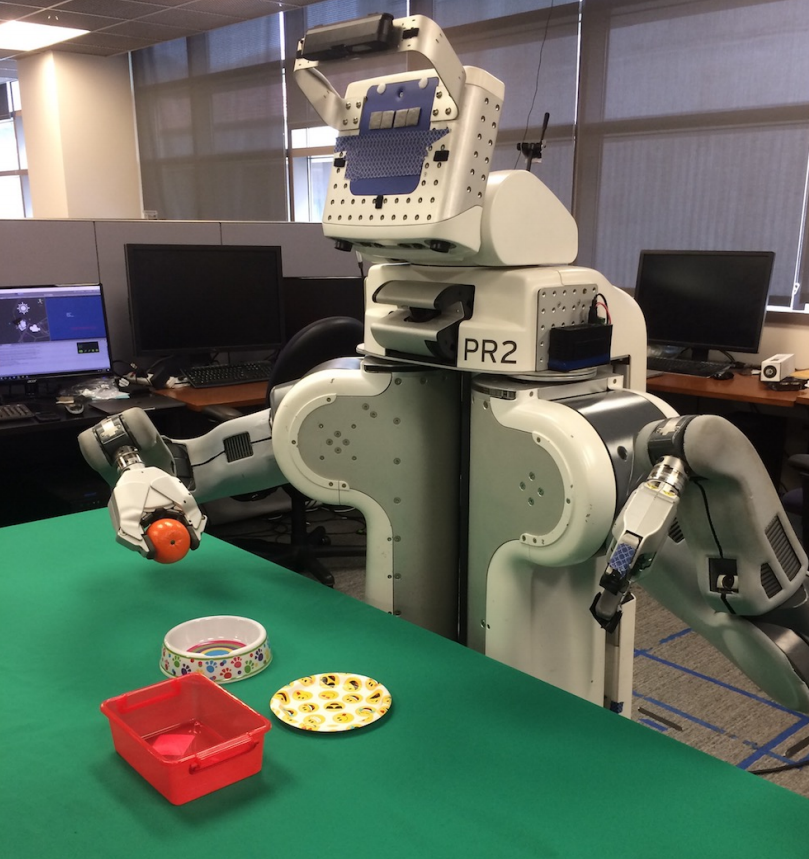
\includegraphics[width=0.9\textwidth]{./chapters/chapter_2/imgs/img_visual_motor_control.png}
            \caption{}
            \label{fig:ch2_visual_motor_control}
        \end{subfigure}
        \begin{subfigure}[b]{0.3\textwidth}
            \centering
            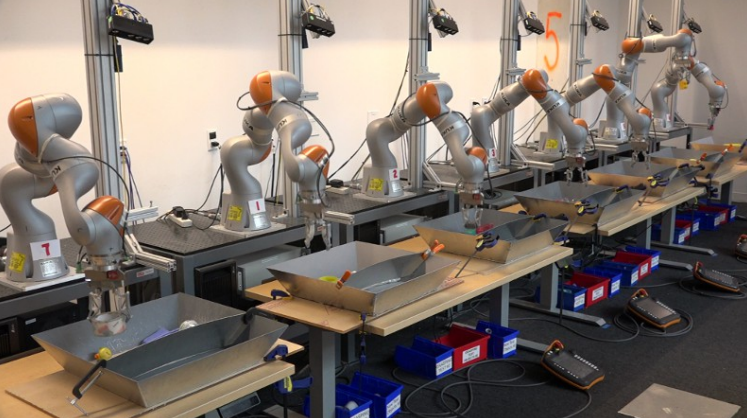
\includegraphics[width=0.9\textwidth]{./chapters/chapter_2/imgs/img_vision_based_robotics.png}
            \caption{}
            \label{fig:ch2_vision_based_robotics}
        \end{subfigure}
        \begin{subfigure}[b]{0.3\textwidth}
            \centering
            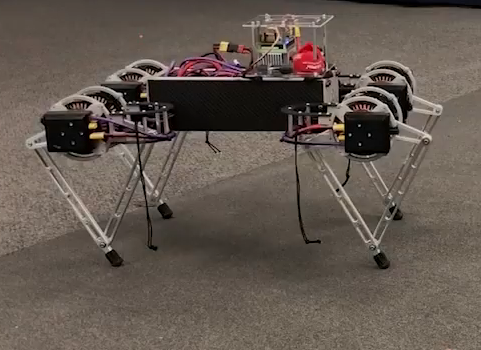
\includegraphics[width=0.9\textwidth]{./chapters/chapter_2/imgs/img_sim_2_real.png}
            \caption{}
            \label{fig:ch2_sim_2_real}
        \end{subfigure}
        \caption{Some DeepRL success stories: (a) PR2 robot learning manipulation tasks [@CITE],
                                              (b) Learning more manipulation tasks using lots of robots [@CITE],
                                              (c) Quadruped running in the real world [@CITE]}
        \label{fig:ch2_drl_stories_3}
    \end{figure}
}

\newcommand{\figMdpSamples}{
    \begin{figure}
        \centering
        \begin{subfigure}[b]{0.9\textwidth}
            \centering
            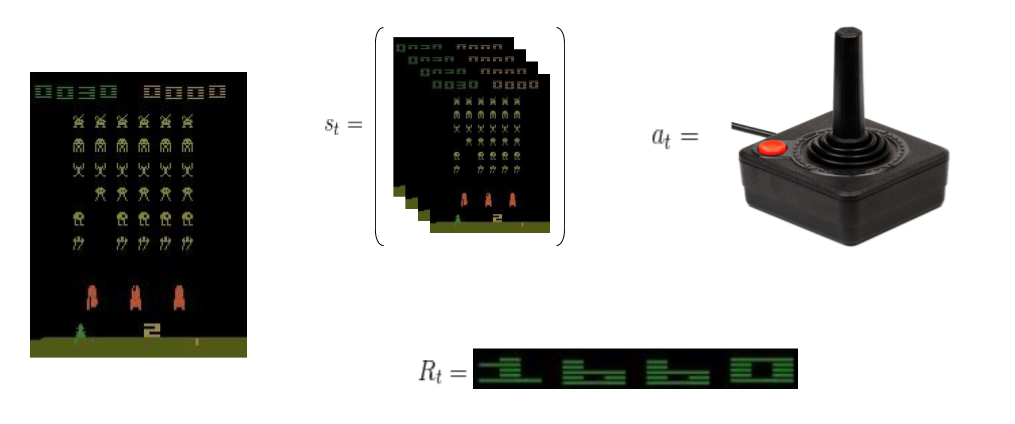
\includegraphics[width=0.9\textwidth]{./chapters/chapter_2/imgs/img_rl_mdp_atari.png}
            \caption{}
            \label{fig:ch2_mdp_sample_atari}
        \end{subfigure}

        \centering
        \begin{subfigure}[b]{0.9\textwidth}
            \centering
            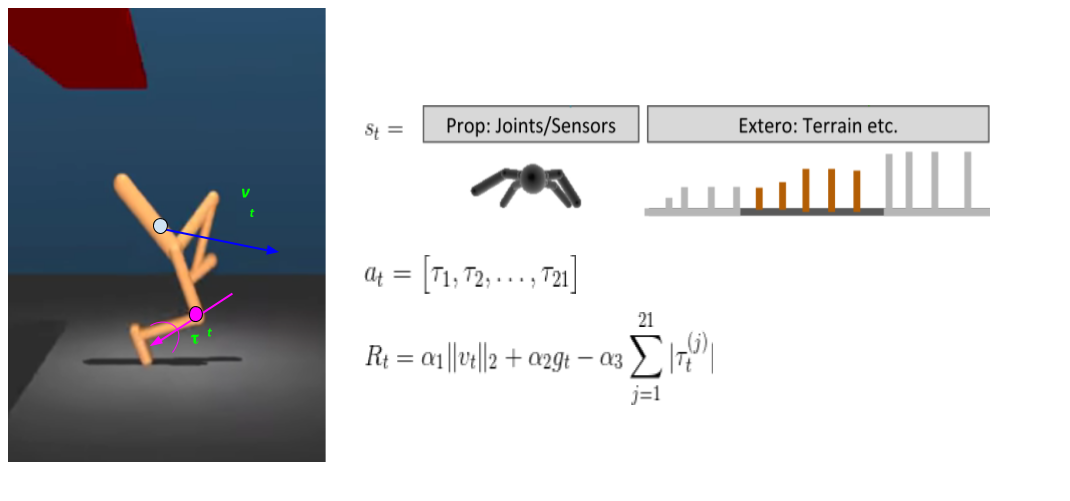
\includegraphics[width=0.9\textwidth]{./chapters/chapter_2/imgs/img_rl_mdp_locomotion.png}
            \caption{}
            \label{fig:ch2_mdp_sample_locomotion}
        \end{subfigure}
        \caption{Some examples of MDPs: (a) MDP modelling an Atari game. 
                                        (b) MDP modelling a locomotion task.}
        \label{fig:ch2_mdps_samples}
    \end{figure}
}

\newcommand{\figRlPolicies}{
    \begin{figure}
        \centering
        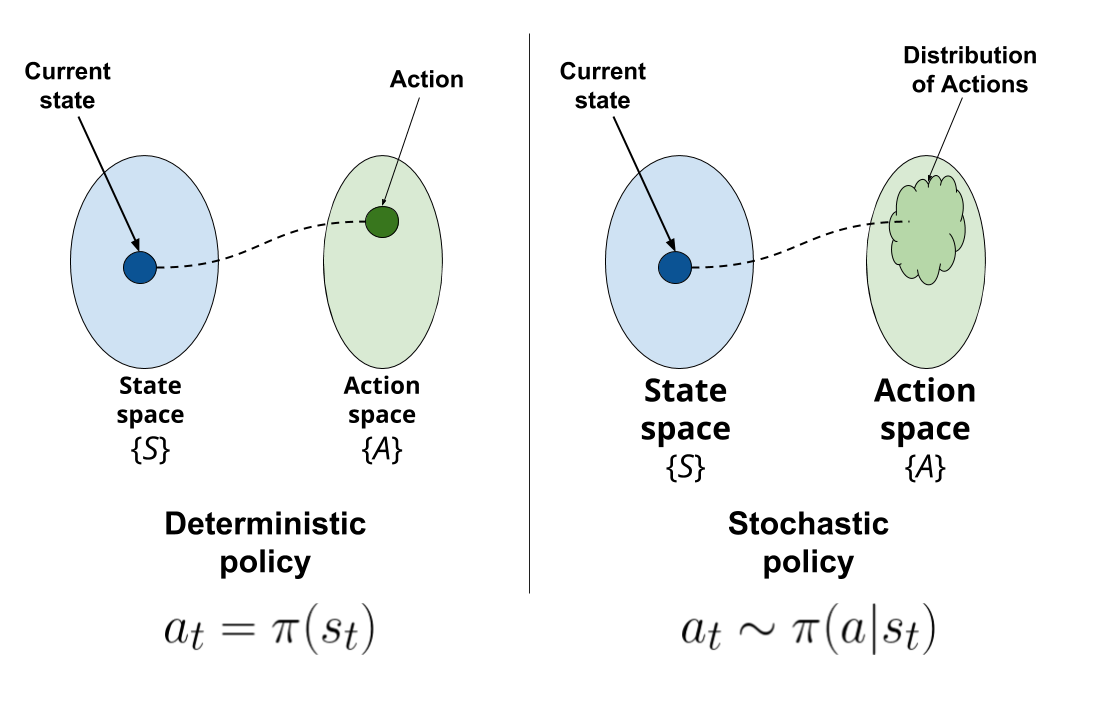
\includegraphics[width=0.9\textwidth]{./chapters/chapter_2/imgs/img_rl_policies.png}
        \caption{Differences between deterministic and stochastic policies.}
        \label{fig:ch2_rl_policies_differences}
    \end{figure}
}

\newcommand{\figRlMethodsLandspace}{
    \begin{figure}
        \centering
        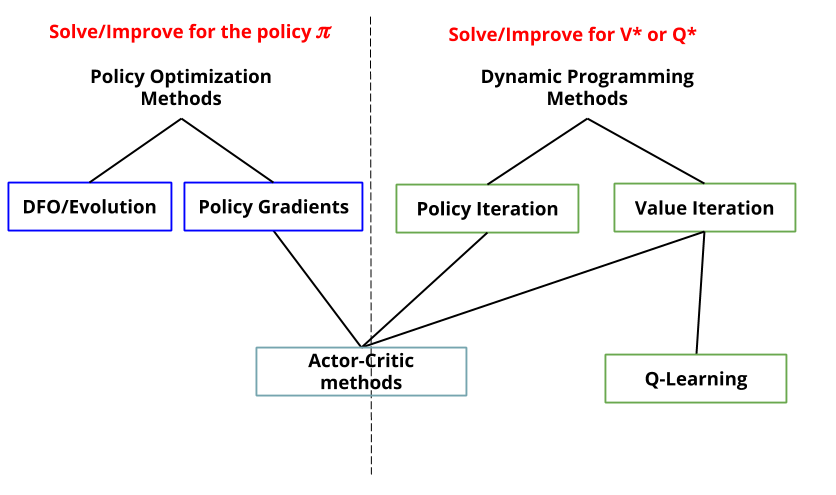
\includegraphics[width=0.9\textwidth]{./chapters/chapter_2/imgs/img_rl_methods.png}
        \caption{RL solution methods landspace. \textbf{Value-based methods} (right) solve for the policy 
                 indirectly, whereas \textbf{Policy-based methods} (left) solve for the policy directly.}
        \label{fig:ch2_rl_policies_differences}
    \end{figure}
}

\newcommand{\figRlPolicyGradientsIntuition}{
    \begin{figure}[!b]
        \centering
        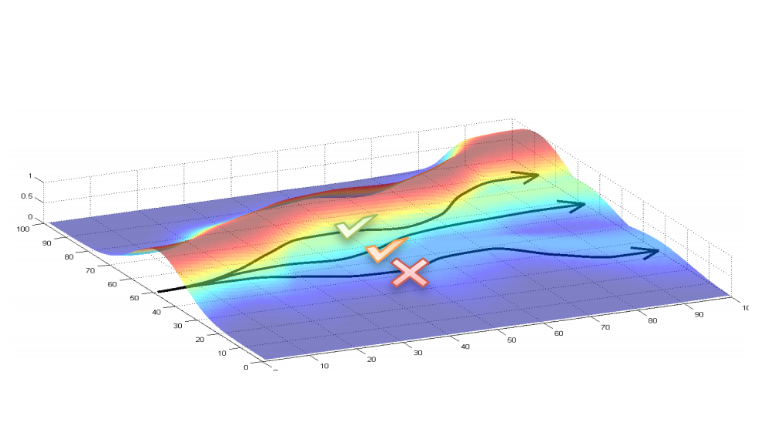
\includegraphics[width=0.8\textwidth]{./chapters/chapter_2/imgs/img_rl_pg_intuition.png}
        \caption{Intuition behind Policy Gradients. Actions that yield good trajectories are encouraged}
        \label{fig:ch2_rl_pg_intuition}
    \end{figure}
}

\newcommand{\figRlPolicyParametrization}{
    \begin{figure}
        \centering
        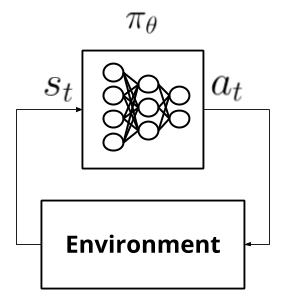
\includegraphics[width=0.3\textwidth]{./chapters/chapter_2/imgs/img_policy_parametrization.png}
        \caption{Parametrization of a policy $\pi$ using a Neural Network}
        \label{fig:ch2_rl_policy_parametrization}
    \end{figure}
}

\newcommand{\figALEgames}{
    \begin{figure}[H]
        \centering
        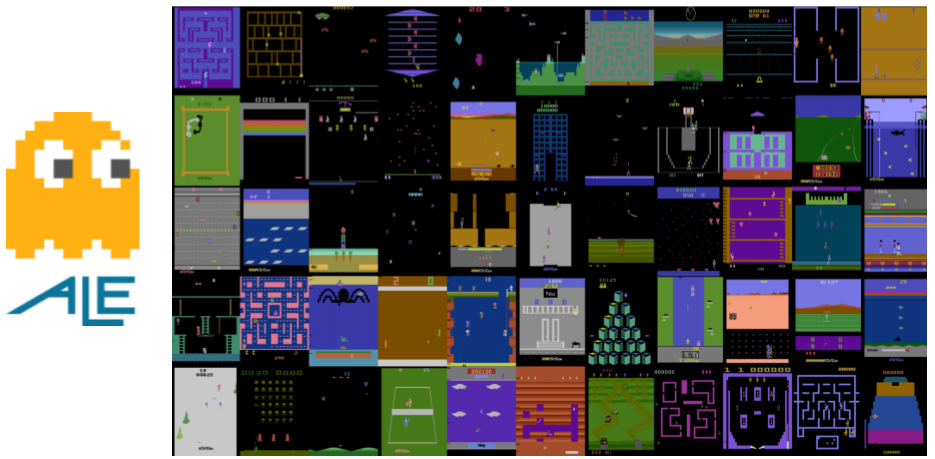
\includegraphics[width=0.6\textwidth]{./chapters/chapter_2/imgs/img_atari_learning_environment.png}
        \caption{Games in the Atari Learning Environment.}
        \label{fig:ch2_ale_games}
    \end{figure}
}

\newcommand{\figOpenAIEnvs}{
    \begin{figure}[H]
        \centering
        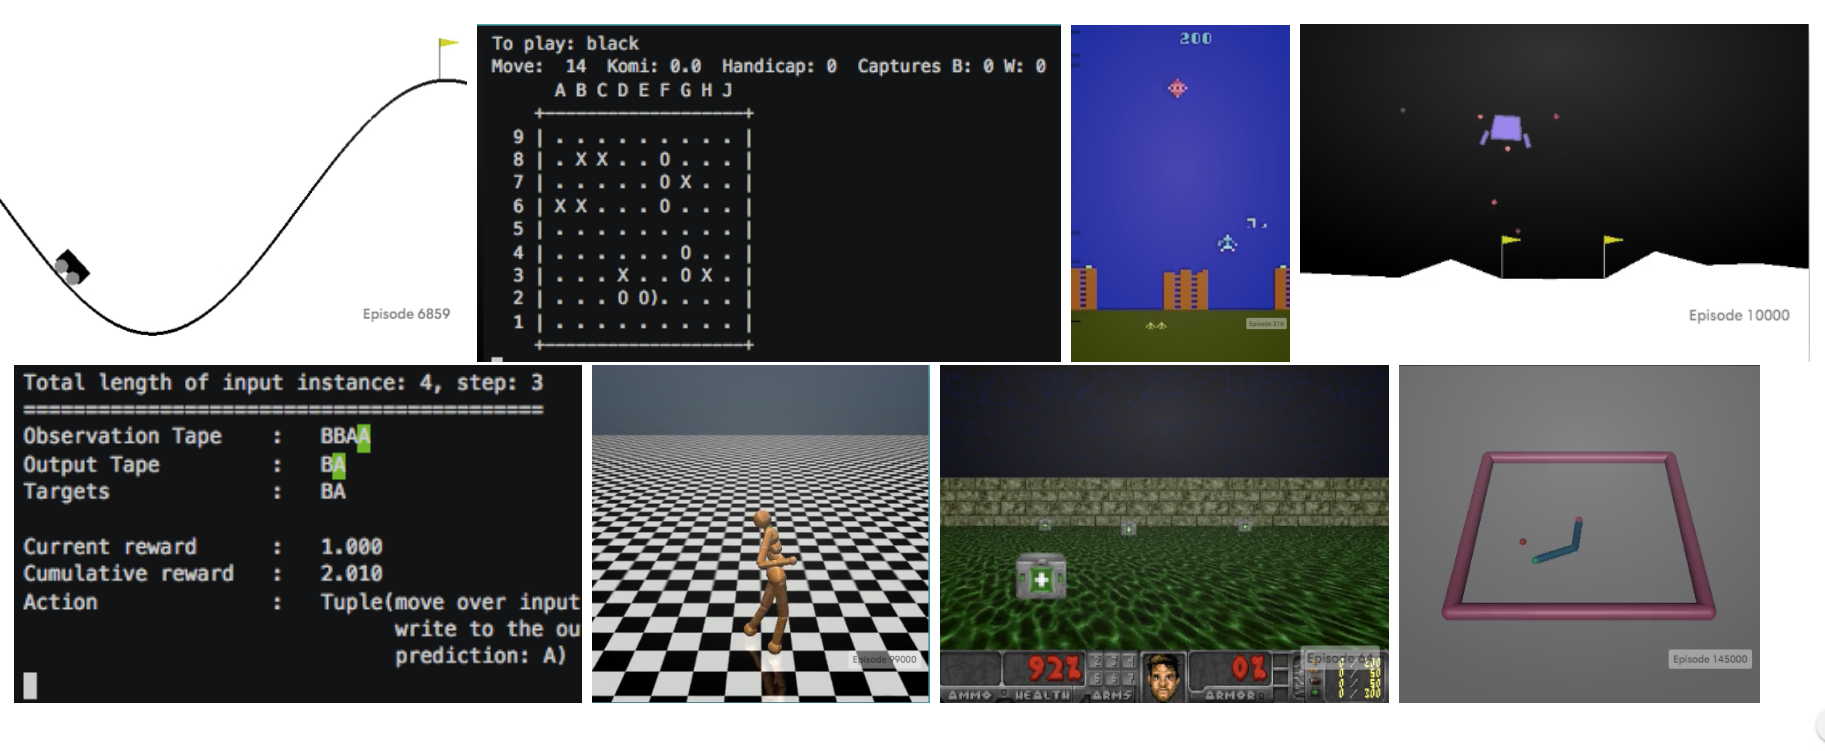
\includegraphics[width=0.9\textwidth]{./chapters/chapter_2/imgs/img_openai_gym_envs.png}
        \caption{Environments in OpenAI Gym.}
        \label{fig:ch2_gym_envs}
    \end{figure}
}

\newcommand{\figDeepmindLabEnvs}{
    \begin{figure}[H]
        \centering
        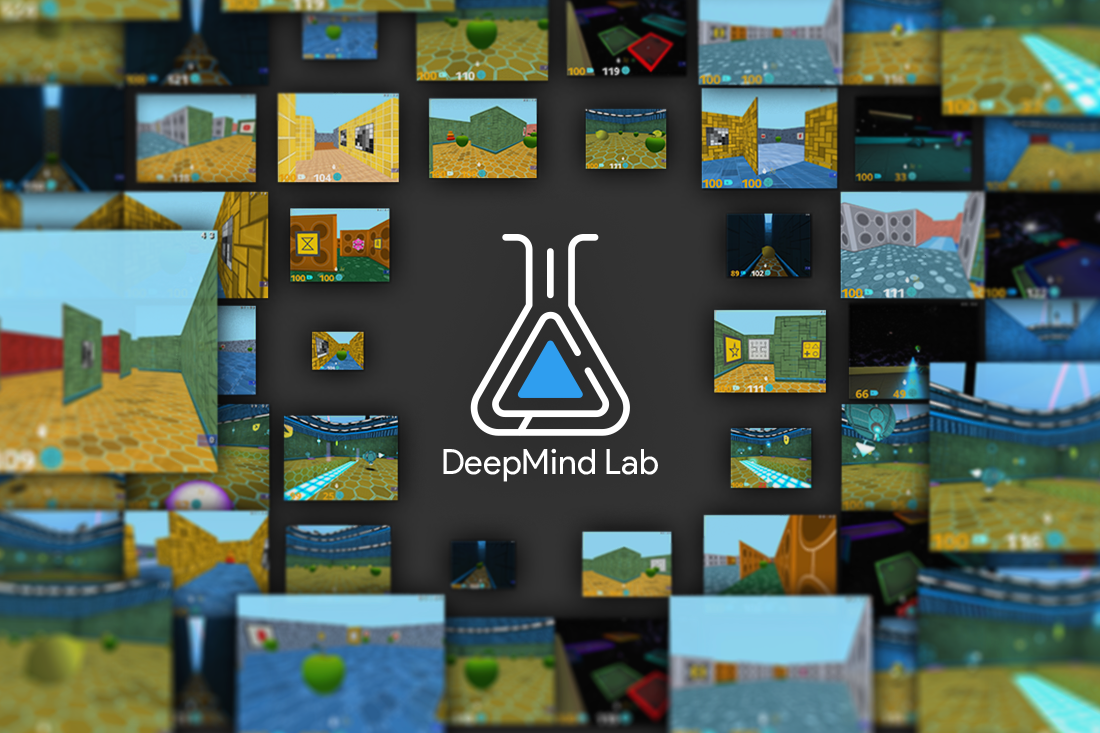
\includegraphics[width=0.7\textwidth]{./chapters/chapter_2/imgs/img_deepmind_lab.png}
        \caption{Environments in Deepmind Lab}
        \label{fig:ch2_deepmind_lab}
    \end{figure}
}

In this chapter we we will give an overview of the core concepts needed to
understand the following chapters in this document. 


\begin{itemize}
    \item We start by giving a \textbf{brief overview of the field of Deep Reinforcement Learning}.
    \item Then we give an overview of \textbf{learning environments}, why are they 
          important and some examples used in current Deep Reinforcement Learning research.
    \item Finally we give a more specific overview of \textbf{learning environments 
          for robot locomotion}, what are their components, and some concepts about their design.
\end{itemize}


\section{Deep Reinforcement Learning}

At a very high level Deep Reinforcement Learning (DRL) could be thought as combination 
of current Deep Learning (DL) models and techniques, with the framework of Reinforcement 
Learning (RL), to solve complex RL problems. This combination has given impressive 
results over the past few years, like being able to play a suite of atari games [@CITE], 
beating the world Go champion [@CITE], making simulated characters develop locomotion
skills [@CITE,@CITE,@CITE], and being able to learning manipulation tasks in real-world
robotics platforms [@CITE], just to name a few.

We will cover most of the core concepts of the Reinforcement Learning framework in 
this section (MDPs, Value based methods). Then we will explain the links between 
Deep Learning and Reinforcement Learning (function approximation, Policy Gradients) and
finally explain some details of some state-of-the-art DRL algorithms.

\subsection{Reinforcement Learning}

Reinforcement Learning is an overloaded term that encloses both a \textbf{learning approach}
and the \textbf{algorithms} that solve problems in this paradigm. RL as a learning approach
is a learning paradigm, like supervised and unsupervised learning, with the difference that
an \textbf{agent} has to \textbf{learn from interaction} with an environment.

\figrlloop

